\section{Experiment Results}
\label{sec:results}
In this section we first evaluate the performance of the object
detecting by combination multi-features
%, and show how they can be used to predict class for new images 
(section 5.1). The comparision of our method with other detecting methods base on the state-of-art
result of PASCAL 2009 is also presented. Finally, the evaluation of automatically
choosing feature for detecting new object is presented in section 5.2.
%We work on seven features: edge, corner, line, circle, HoG, SURF, and color. 
\subsection{Detection result}
We create the edge image-$I_E$ and corner
image-$I_C$ for an input image. We use Canny edge detector with 3x3-structure, and Harris corner detector with 5x5 structure. Beside, Gaussian filter is applied on input image before detecting edge and corner to subtract background.

\textit{Edge map satisfaction:} Let denote $n_{1}^{e}$ as the number of edges in the edge image $I_E$; and $n_{2}^{e}$ as the number of edges matchings between $I_E$ and $M_E$.
The degree of satisfying $M_E$ of $I_E$ is determined by some conditions as
bellow:
\begin{equation}
 \begin{array}{rcl}
   C_1^E(I_E) = \left\{ 
   \begin{array}{rcl}
   1 &  n_2^e > N_1^e \\
   0 &  else
   \end{array}\right. &
   C_2^E(I_E) = \left\{ 
    \begin{array}{rcl}
    1 &  \frac{n_2^e}{n_1^e} > \theta^e \\
    0 & else
    \end{array}\right. \\
   
   C_3^E(I_E) = \left\{ 
   \begin{array}{rcl}
   1 & n_1^e < N_2^e \\
   0 & else
   \end{array}\right. &
   \mbox{~~~~~}
 \end{array}
  \label{eq:edge_map_satisfy}
\end{equation}
where $N_1^e$, $N_2^e$ are constants and $\theta^e$ is a given threshold.
$C_1^E(I_E)$ guaranties that edges in the input image must be in the correct
position to construct object like edges in $M_E$. While both $C_2^E(I_E)$ and $C_3^E(I_E)$
are aiming at avoiding the situation of too much edges representing in the input image. If $Q_E = C_1^E(I_E) \wedge C_2^E(I_E) \wedge C_3^E(I_E)$ is true, then $I_E$ satisfies $M_E$; and the image will be passed to the next corner test step.
But, as we mention in section 3.1, after detecting edge we cannot
know exactly individual edge. It also means that we cannot calculate $n_1^e$ and $n_2^e$. However, instead of counting number of edges, we can sum of pixels which are marked as edge. Thus, $n_1^e$ and $n_2^e$ can be known approximately as:
\begin{equation}
 n_1^e \approx \frac{1}{255} \sum I_E(x,y);
 \mbox{}
 n_2^e \approx \frac{1}{255^2} \sum I_E(x,y)\cdot M_E(x,y)
   \label{eq:n_1_e_and_n_2_e}
\end{equation}
\textit{Corner map satisfaction:} 
Similar to edge test step, we here also define three coditions
\begin{equation}
  \begin{array}{rcl}
   C_1^C(I_C) = \left\{ 
    \begin{array}{rcl}
    1 & n_2^c > N_1^c \\
    0 & else
    \end{array}\right. &   
   C_2^C(I_C) = \left\{ 
    \begin{array}{rcl}
    1 &  \frac{n_2^c}{n_1^c} > \theta^c \\
    0 & else
    \end{array}\right.  \\  
   C_3^C(I_C) = \left\{ 
    \begin{array}{rcl}
    1 & n_1^c < N_2^c \\
    0 & else
   \end{array}\right.  & 
   \mbox{~~~~}
  \end{array}
  \label{eq:corner_map_satisfy}
\end{equation}
where $N_1^c$, $N_2^c$ are constants, $\theta^c$ is a given threshold. $n_1^c$ is the 
the number of corners in the input corner image $I_C$ and $n_2^c$ is the number
of corner matching between $I_C$ and the corner map $M_C$.
\begin{equation}
 n_1^c \approx \frac{1}{255} \sum I_C(x,y);
 \mbox{}
 n_2^c \approx \frac{1}{255^2} \sum I_C(x,y)\cdot M_C(x,y)
   \label{eq:n_1_e_and_n_2_e}
\end{equation}
The qualification of satisfying the corner map is determined by the criterion $Q_C = C_1^C(I_C) \wedge C_2^C(I_C) \wedge C_3^C(I_C)$

\textit{Orientation satisfaction:}
The orientation of each pixel is calculated by using HOG descriptor method as in~\cite{bay2008surf}. The magnitude $m(x, y)$
and the orientation $\theta(x, y)$ are computed as
%\begin{eqnarray*}
\begin{equation}
    m(x,y) = \sqrt{{g_x(x,y)}^2 + {g_y(x,y)}^2}
    \mbox{~;~}
    \theta(x,y) = \arctan(\frac{g_x(x,y)}{g_y(x,y)})
\end{equation}
%\end{eqnarray*}
where $g_x(x, y)$ and $g_y(x, y)$ denotes the $x$ and $y$ components of the
image gradient in $x$ and $y$ direction calculated by $1-D$ centered mask $[ 1, 0, 1]$
\begin{equation}
    \begin{array}{rcl}
    g_x(x,y) = I(x+1,y) - I(x-1,y) \\
    g_y(x,y) = I(x,y+1) - I(x,y-1)
    \end{array}
\end{equation}
After that, we specify some sub regions where the
orientation such as horizontal, vertical and diagonal is very strong.
\begin{figure}[ht]
  \centering
  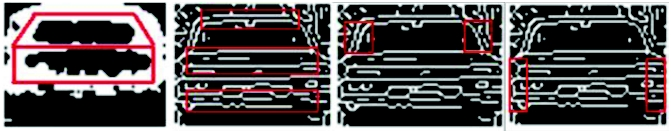
\includegraphics[width=3.15in]{images/hog.jpg}
  \caption{Sub regions with strong orientation of front/rear view car, from left to
right: edge image, horizontal, diagonal and vertical.}
  \label{fig:hog}
\end{figure}
The orientation is ranged in $[0, 2\pi]$, divided into $16$ bins: $h[0]...
h[15]$. For each sub region, we calculate histogram of orientation in
that region by quantizing the orientation $\theta(x, y)$ for all pixels falling
to $h[i]$ bins, $i=\overline{0,15}$, weighted by its magnitude $m(x, y)$.
Condition for input image satisfies orientaiton is that
\begin{equation}
    \begin{array}{rcl}
   H(S) = \left\{ 
   \begin{array}{rcl}
   1 & \mbox{~~} & \frac{h[0] + h[15] + h[7] + h[8]}{\sum_{i=0}^{15}h[i]} > \sigma_1\\
   0 & \mbox{~~} & else
   \end{array}\right. \\
   V(S) = \left\{ 
   \begin{array}{rcl}
   1 & \mbox{~~} & \frac{h[3] + h[4] + h[11] + h[12]}{\sum_{i=0}^{15}h[i]} > \sigma_2\\
   0 & \mbox{~~} & else
   \end{array}\right. \\
   D(S) = \left\{ 
   \begin{array}{rcl}
   1 & \mbox{~~} & \frac{h[1] + h[2] + h[9] + h[10]}{\sum_{i=0}^{15}h[i]} > \sigma_3\\
   0 & \mbox{~~} & else
   \end{array}\right. 
    \end{array}
\end{equation}
where $\sigma_1$, $\sigma_2$, and $\sigma_3$ are specific thresholds. If all sub-regions satisfy
conditions of the strong orientation respectively then input image
satisfies orientation.

Our proposed scheme is evaluated on eight object-categories,
including front/rear view car, side view car, bicycle, train, aeroplane,
motorbike, sheep and horse. We use CALTECH256, UIUC and
PASCAL-VOC 2010 database. Beside, in order to evaluate the result
more exactly, an additional about 1500 negative examples are
collected randomly and added to the database. Thus with each
object-category, the whole database contains about more than 1500
negative images and 1500 positive images (including 1000 images
for training, and 500 images for testing).
%The database contains natural images that are taken from several sources and include occlusion and cluttered backgrounds. 
%With side view car, images used for training have the same size 40x100 as in original database. Otherwhile, all images in the training set of front/rear view car, we resize manually into $60\times80$ to eliminate the influence from background. Similar to other object, 
In the training stage, we choose the basic size for every object. But in the detecting
phase, with an input image, we preprocess it by resizing it into four
times as size of the training image. After detecting at this scale, we reduce it size and continue detect
until the size equals to the training image. By doing that, it is able to
detect all objects in the input image even if the size of object in it is
smaller or larger than the basic size, although it consumes more time
than detecting at a specific scale.
%\small
%\begin{tabular}{p{3.5cm}p{8cm}p{5cm}}
\begin{table}[htbp]
\small
\begin{tabular}{c}%p{3.5cm}p{8cm}p{5cm}}
   \begin{tabular}{|c|c|c|c|c|c|} \hline
	Set & No. image & Correct & In-correct & False rate & Accuracy \\ \hline
	Calt 101 & 504 & 481 & 23 & 4.57\% & 95.43\% \\ \hline
	Calt 256 & 526 & 475 & 41 & 8.95\% & 92.05\% \\ \hline
	Non- car & 665 & 624 & 41 & 6.17\% & 93.83\% \\ \hline
	\end{tabular} \\ %\hline
	Detection result of front/rear view car \\ %\hline
	\begin{tabular}{|c|c|c|c|c|c|} \hline	
	Set & No. image & Correct & In-correct & False rate & Accuracy \\ \hline
	UIUC1 & 300 & 275 & 25 & 8.33\% & 91.67\% \\ \hline
	UIUC2 & 278 & 264 & 14 & 5.04\% & 94.96\%  \\ \hline
	Non- car & 665 & 638 & 27 & 4.06\% & 95.94\% \\ \hline
	\end{tabular} \\ %\hline 
	Detection result of side view car \\ %\hline
\end{tabular}
\caption{The result of our car detecting system.}
\label{table:car_detecting_result}
\end{table}
The final result of our system for car detection is shown in table~\ref{table:car_detecting_result}. The performance of Zhenfeng Zhu~\cite{zhu2004car} (with the same database: Caltech and UIUC) reaches the highest accurate rate at $90.5\%$, while
the lowest accurate of our sytem is about $91.67\%$. This shows that our schema get a better perfomance. Some examples of correct/incorrect detection are shown in Fig~\ref{fig:bicyle_plane_example}. 
%The last image in Fig. 9 presents the positive false of bicycle, while in Fig. 10 it is the negative false of areo plane.
\begin{figure}[ht]
  \centering
  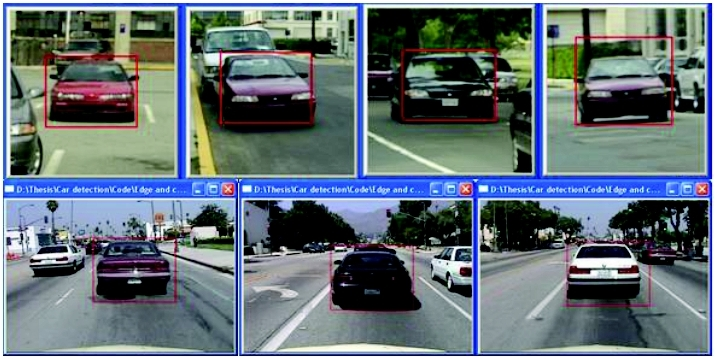
\includegraphics[width=3.15in]{images/car_example.jpg}
  \caption{The true positive detection with front/rear view car.}
  \label{fig:car_example}
\end{figure}
\begin{figure}[ht]
  \centering
  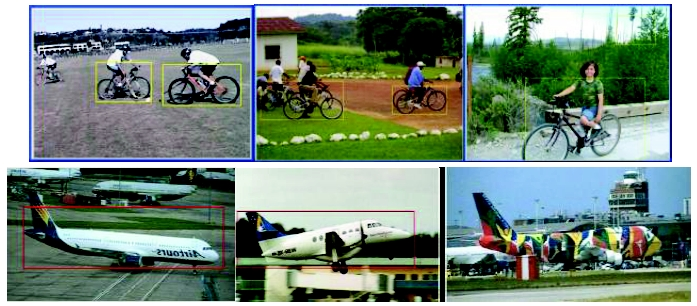
\includegraphics[width=3.15in]{images/bicycle_plane_example.jpg}
  \caption{Bicyle (top) and areoplane (bottom) detection result.}
  \label{fig:bicyle_plane_example}
\end{figure}
We use two ways to check if edge/corner pixel is at right position or
not. One is that if no-pixel in map and no-pixel in mage, then result
is not right $(0\times 0=0)$; other is that no-pixel in map, no-pixel in image,
the result is between right and not-right $(0\times 0=0.5)$. Because if there
is no-pixel in map and no-pixel in testing image, it mean that there
is no edge/corner at that position. That is also a good hint for
regconize object. The final average precision (AP), average recall
(AR) of these two methods is shown in table~\ref{table:compare_0_5}.
%\begin{table}[htbp]
%\small
%\begin{tabular}{|c|c|c|}%p{3.5cm}p{8cm}p{5cm}} 
%    \hline
%	Object & 
%	  \begin{tabular}{c} \hline
%	  $0\times 0 = 0$ \\ \hline
%		  \begin{tabular}{c|c} \hline
%		   AP & AR \\ \hline
%		  \end{tabular}	  
%	  \end{tabular} &
%	  \begin{tabular}{c} 
%	  $0\times 0 = 0.5$ \\ \hline
%		  \begin{tabular}{c|c} \hline
%		   AP & AR \\ \hline
%		  \end{tabular} 
 %	  \end{tabular}  \\ \hline
%\end{tabular}
%\caption{The result of our car detecting system.}
%\label{table:car_detecting_result}
%\end{table}
\begin{table}[htbp]
\small
\begin{tabular}{|c||c|c||c|c|}%p{3.5cm}p{8cm}p{5cm}} 
    \hline 
     Object &  AP (0x0=0) & AR(0x0=0) & AP (0x0=0.5)  & AR(0x0=0.5)  \\ \hline 
     F/r car & 97.40\% & 89.71\% & & \\ \hline
     Side car & 95.83\% & 92.38\% & & \\ \hline
	 Bike & 83.76\% & 72.64\% & 83.82\% & 78.46\% \\ \hline
	Train & 84.05\% & 74.10\% & 81.57\% & 76.43\% \\ \hline
	Aero plane & 85.59\% & 87.56\% & 81.15\% & 86.54\% \\ \hline
	Motorbike & 95.63\% & 85.35\% & 95.35\% & 84.47\% \\ \hline
	Horse & 88.64\% & 68.78\% & 88.37\% & 70.72\% \\ \hline
	Sheep & 74.84\% & 65.96\% & 86.13\% & 71.93\% \\ \hline 
\end{tabular}
\captionof{table}{Comparision between $0\times 0=0$ and $0\times 0=0.5$}
\label{table:compare_0_5}
\end{table}
If there are many edge/corner inside object (such as aero plane,
motorbike), then the $0\times 0=0$ method is better. Otherwhile, if object
doesn t include a lot of edge/corner (bike, horse, sheep or animal is
example), the $0\times 0=0.5$ method will get the higher perfomance. In the
case there are a few of edge/corner on the surface of object (ex.
train), both $0\times 0=0$ and $0\times 0=0.5$ do the same function, and the result
is not different so much.
\subsection{Automatic feature selection for object detecting}
In our experiments below we evaluate the performance of
automatically choosing semantic attribute features on the large data
set used in the 2009, 2010 PASCAL VOC challenge. We believe this
is the first time that the performance of automatically choosing
features has been tested on a standard object classification
benchmark.
In previous section, our system can detect eight categories with
satisfactory result. We combine many features for every object. But
which one category, we must decide which feature is used for
detecting by ourselves. For example, to detect a bike, circle feature is
a good choice, because most of bikes have two wheels with circle
shape. With horse or sheep ojbect, color is a good hint 
due to the fact that the color space of horse or sheep does not change dramatically. With SURF and HoG
feature, because these features are not visual, it is difficult to determine they are suitable for one object or not. In this part, we will evaluate our proposed method in section $4$ for automatically choosing features. We first test with seven features:
edge, corner, HoG, cirle, line, SURF and color. Bias $\omega_p$ and $\omega_n$ are set to $0.6$ and $0.4$ respectively.
\begin{table}[htbp]
\small
\begin{tabular}{|c|c|c|c|c|c|c|c|}%p{3.5cm}p{8cm}p{5cm}} 
    \hline
    Object & Edge & Corner & Line & Circle & HoG & SURF & Color \\ \hline
	F/r car & 1 & 1 & 0 & 0 & 1 & 1 & 0  \\ \hline
	Side car & 1 & 1 & 0 & 1 & 1 &  1 & 0  \\ \hline
	Bike & 1 & 1 & 1 & 1 & 0 & 0 & 0  \\ \hline
	Train & 1 & 1 & 0 & 0 & 1 & 1 & 0  \\ \hline
	Aero plane & 1 & 1  & 1 & 0 & 0 & 1 & 0  \\ \hline
	Motorbike & 1  & 1 & 0 & 0 & 0 & 1 & 1  \\ \hline
	Horse & 1 &  1 & 1 & 0 & 0 & 1 & 1  \\ \hline
	Sheep & 1 & 1 & 0 & 0 & 0 & 1 & 1  \\ \hline
	Tower & 1 & 1 & 1 & 0 & 1 & 0 & 0  \\ \hline
	Flower & 1 & 1 & 0 & 0 & 1 & 1 & 0  \\ \hline
\end{tabular}
\captionof{table}{Object with automatically chosen features}
\label{table:auto_feature_select}
\end{table}
Result of automatically choosing features is in table~\ref{table:auto_feature_select}, where
zero$(0)$ means that feature is not good for object, and one$(1)$
represents we should use this feature to detect object. The image
database for testing automatically choosing feature is same with the
image database for object detecting in section 5.1. The outcome of
this algorithm is predictable, it is almost fit with what we have done
by hand. Only one thing is not as we though is that color feature is
useful for motorbike object (value $1$ at the cell of column Color and
row Motorbike). After checking the motorbike database, we
recognize that most of motorbike-images from CALTECH 256 have
white background and their colors only vary in green, brown, red.
That is the reason why with this database, color is helpful for
detecting motorbike object.
\begin{figure}[ht]
  \centering
  \includegraphics[width=3.35in,height=1.2in]{images/output.pdf}
  \caption{Satisfied, positive and negative score of horse object(left) and side view car(right) .}
  \label{fig:auto_selection}
\end{figure}
In the fig~\ref{fig:auto_selection}, detail of automatically choosing feature for
horse object and side view car object is described. 
%From set of features, we choose one feature with the highest satisfied score (calculated as in section 4). We combine every feature with the first chosen feature, and then we recalculate the satisfied score. We will pick the feature which makes the satisfied score maximum. This feature then is moved to chosen feature set. Next running time, both two chosen features are integrated with new one to compute new satisfied score. By doing this way, 
%The satisfied score increases slowly until it rises to a superior value, which is the maximum value. After that, if more features are combined, the result will be worse. If the score is lower than previous continuously in three permutations, our algorithm would be terminated, and reverse to the peak of score. 
At the beginning, with only one feature, generally the positive score $ pos(f_i,F_c) = |sat(F_c \cup \{f_i\}|T_{pos})| * 1/|T_{pos}|$  is very large because the most of images in $T_{pos}$ satisfy
this feature. Other while, the negative score $neg(f_i,F_c) = (|T_{neg}| - |sat(F_c \cup \{f_i\}|T_{neg})| * 1/|T_{neg}|$ is small. When the more features are
added to chosen feature set, the smaller positive score is, and the
larger negative score becomes. Totally, the satisfied score $g(f_i,F_c) = \omega_p * pos(f_i,F_c) + \omega_n * neg(f_i,F_c)$ (with $\omega_p = 0.6$ and $\omega_n = 0.4$), increases
slowly until it rises to a superior value, represented by the red line. After
this peak, if more features are integrated into $F_C$, the satisfied score
gets lower value.
If the score is lower than the previous one continuously in $k$ permutations, our algorithm would be terminated, and reverse to the peak of score (in our
evaluation, k = 3). Only features before the score gains the peak (on the left side of the red line) will be chosen as strong representative features for that object. For example, with horse object these are chosen-features: CL(color), C(corner), L(line), E(edge) and S(SURF). Other while, with side-view car, H(HoG) is the best feature following by E(edge), CR(circle), E(edge) and C (corner).







